\subsection{Critiques of RSVP}
In order to test how efficient RSVP actually is, a study was conducted by \citeA{schotter_dont_2014}. One thing that is criticized with RSVP techniques is the ability to go back and re-read words for improving one's comprehension. This process is called \textit{regression}, and according to \citeauthor{schotter_dont_2014} about 10\% to 15\% of the time spent reading is by making regressions, i.e. moving eyes back in the text to read material that has previously been processed. The hypothesis is that regression supports reading comprehension, since it allows readers to access more information from the text. This is especially true with texts that are more difficult to read, i.e. that it requires the reader to go back and read words again to make sense of how the sentence is structured. Readers are more likely to make a regression when they sense that their comprehension of the sentence has faltered \cite{schotter_dont_2014}.

By using trailing-mask conditions in their experiment, meaning that whenever a person has read a word, it becomes unreadable by changing it to X's instead, \citeA{schotter_dont_2014} could measure the effects of RSVP (i.e., being shown one word at a time - see Figure \ref{fig:trace_cross}). They found evidence that support the importance of regression. They used a combination of simple sentences and ambiguous garden-path sentences (e.g., "While
the man drank the water that was clear and cold overflowed from the toilet") to investigate when participants tended to regress the most, as well as measure their reading comprehension by answering questions about the sentences. \citeauthor{schotter_dont_2014} found that restricting the opportunity to re-read words with the trailing-mask (replacing the letters with X's) decreased comprehension globally. Unsurprisingly, they also found that participants were significantly more likely to regress in ambiguous sentences, since they had to go back and re-read to understand the sentence properly. Participants made regressions to go back and search for information that would support their overall understanding of the given text. \citeauthor{schotter_dont_2014} also saw evidence that suggests that participants were able to suppress the tendency to re-read, when they knew that regression was not possible due to the trailing-mask system.

\begin{figure}[htbp]
\centering
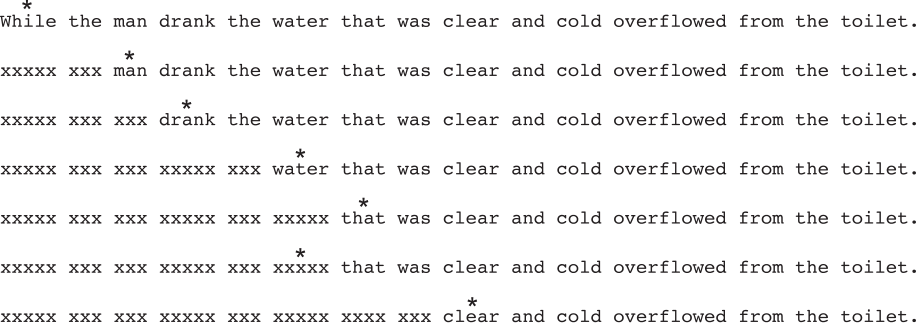
\includegraphics[width=0.45\textwidth]{Pics/trace_crosses}
\caption{\protect\citeauthor{schotter_dont_2014} used eye-tracking to mask the words a person had already read, making it impossible to regress. Asterisks represent eye fixations.}
\label{fig:trace_cross}
\end{figure}

\citeauthor{schotter_dont_2014} conclude that reading without the ability to re-read parts of the text, decreases the comprehension accuracy and leads to a poorer understanding of the text.

%\textbf{Loss of spatial awareness and formatting}

(INSERT REF) suggests some improvements that should be made to RSVP. One improvement is that it should only present samples of the text, e.g. by selecting only the most informative words of a sentence. This could be determined by only presenting the least frequent content words as well as critical function words. (INSERT REF) also suggests that the duration each word is presented, should be based on an estimate of the processing time for the word. Spritz calculates an estimate by using the shape of the word as well as the length of the word(INSERT SPRITZ REF), however there might be different theories on how to calculate this \textbf{(Maybe find a better way to write this)}.

%% by Gustav:
\citeA{baker_is_2005} conducted a study to investigate different layouts when reading online. He found that depending on the reader and the context, different ways of formatting the text were preferred. Longer lines generally facilitate faster reading speeds, while shorter lines can result in increased reading comprehension. Additionally, reading speeds are faster for both single and multiple columns, but there is a preference for multiple short columns with 45-65 number of characters per line being the optimal. The results suggest that there is not a one best way to present text online, but that faster readers performed best when reading two-column texts. Slower readers benefited more from single-column layouts \cite{baker_is_2005}.